% answers.tex —— 2014 年全国Ⅰ卷（理科） · 参考答案与详细解析片段
% 由 tools/generate_projects.py 依来源总账自 2014/2014_数学真题_全国1理_试题.md + 2014/2014_数学真题_全国1理_解析正文.md + 2014/2014_数学真题_全国1理_答案要点.md 生成，勿手改（改源 MD 后重跑）


\begin{gktip}
固定源 PDF 是印刷页码 899–900 的两页题面，不附答案或解析。以下各题均依据题面独立复算，\textbf{非官方标准答案}；第 6、7、12、18、19、22 题图形在 LaTeX 工程中以 TikZ/PGFPlots 矢量源重绘。
\end{gktip}

\gkpart{一、选择题}

\begin{answer}
\gksolhead{1}{}

\textbf{题目}：

已知集合 $A=\{x\mid x^2-2x-3\geqslant0\}$，$B=\{x\mid-2\leqslant x<2\}$，则 $A\cap B=$\mbox{（　　）}

（A）$[-2,-1]$　　（B）$[-1,2)$　　（C）$[-1,1]$　　（D）$[1,2)$

\Needspace{4\baselineskip}
\textbf{解析}

$x^2-2x-3=(x-3)(x+1)$，故 $A=(-\infty,-1]\cup[3,+\infty)$。与 $B=[-2,2)$ 取交集得 $[-2,-1]$。

\gkanswer{答案：A}

\end{answer}
\begin{answer}
\gksolhead{2}{}

\textbf{题目}：

$\dfrac{(1+i)^3}{(1-i)^2}=$\mbox{（　　）}

（A）$1+i$　　（B）$1-i$　　（C）$-1+i$　　（D）$-1-i$

\Needspace{4\baselineskip}
\textbf{解析}

\nopagebreak[4]
\[
\frac{(1+i)^3}{(1-i)^2}=\frac{-2+2i}{-2i}=-1-i.
\]

\gkanswer{答案：D}

\end{answer}
\begin{answer}
\gksolhead{3}{}

\textbf{题目}：

设函数 $f(x),g(x)$ 的定义域都为 $\mathbb R$，且 $f(x)$ 是奇函数，$g(x)$ 是偶函数，则下列结论正确的是\mbox{（　　）}

（A）$f(x)g(x)$ 是偶函数　　（B）$|f(x)|g(x)$ 是奇函数

（C）$|g(x)|f(x)$ 是奇函数　　（D）$|f(x)g(x)|$ 是奇函数

\Needspace{4\baselineskip}
\textbf{解析}

$|g(x)|$ 仍为偶函数，故 $|g(x)|f(x)$ 为奇函数；其余选项所述奇偶性不成立。

\gkanswer{答案：C}

\end{answer}
\begin{answer}
\gksolhead{4}{}

\textbf{题目}：

已知 $F$ 是双曲线 $C:x^2-my^2=3m (m>0)$ 的一个焦点，则点 $F$ 到 $C$ 的一条渐近线的距离为\mbox{（　　）}

（A）$\sqrt3$　　（B）$3$　　（C）$\sqrt{3m}$　　（D）$3m$

\Needspace{4\baselineskip}
\textbf{解析}

\Needspace{5\baselineskip}
将方程化为 $\dfrac{x^2}{3m}-\dfrac{y^2}{3}=1$。焦点为 $(\sqrt{3(m+1)},0)$，一条渐近线可写为 $x-\sqrt m\,y=0$，焦点到此线的距离为

\nopagebreak[4]
\[
\frac{\sqrt{3(m+1)}}{\sqrt{1+m}}=\sqrt3.
\]

\gkanswer{答案：A}

\end{answer}
\begin{answer}
\gksolhead{5}{}

\textbf{题目}：

$4$ 位同学各自在周六、周日两天中任选一天参加公益活动，则周六、周日都有人参加公益活动的概率为\mbox{（　　）}

（A）$\dfrac18$　　（B）$\dfrac38$　　（C）$\dfrac58$　　（D）$\dfrac78$

\Needspace{4\baselineskip}
\textbf{解析}

四人任选同一天的情形有 $2$ 种，各自概率为 $(1/2)^4$。所求概率为 $1-2\times(1/2)^4$。

\gkanswer{答案：D}

\end{answer}
\begin{answer}
\gksolhead{6}{}

\textbf{题目}：

如图，圆 $O$ 的半径为 $1$，$A$ 是圆上的定点，$P$ 是圆上的动点，角 $x$ 的始边为射线 $OA$，终边为射线 $OP$，过点 $P$ 作直线 $OA$ 的垂线，垂足为 $M$，将点 $M$ 到直线 $OP$ 的距离表示为 $x$ 的函数 $f(x)$，则 $y=f(x)$ 在 $[0,\pi]$ 上的图象大致为\mbox{（　　）}
\nopagebreak[4]
\begin{center}% 2014 全国卷Ⅰ理科第 6 题：圆、垂足与四个函数图像选项。
\begin{tikzpicture}[font=\scriptsize,>=Stealth,line cap=round,line join=round]
  % 题干圆图：OA 为始边，OP 为终边，PM 垂直 OA。
  \begin{scope}
    \coordinate (O) at (1.4,1.25); \coordinate (A) at (3.4,1.25);
    \coordinate (P) at (2.78,2.70); \coordinate (M) at (2.78,1.25);
    \draw (O) circle (2); \draw[->] (O)--(A); \draw[->] (O)--(P); \draw (P)--(M);
    \node[below left] at (O) {$O$}; \node[right] at (A) {$A$};
    \node[above] at (P) {$P$}; \node[below] at (M) {$M$};
    \draw (O) ++(.55,0) arc[start angle=0,end angle=46,radius=.55] node[midway,right] {$x$};
  \end{scope}
  % 选项共用坐标轴语义；实线曲线对应源面。
  \begin{scope}[xshift=5.3cm,yshift=2.35cm]
    \draw[->] (0,0)--(3.55,0) node[right] {$x$}; \draw[->] (0,-.25)--(0,1.55) node[above] {$y$};
    \draw (0,.96)--(.12,.96) node[left] {$1$}; \node[below left] at (0,0) {$O$}; \node[below] at (3,0) {$\pi$};
    \draw[line width=.55pt] plot[smooth] coordinates {(0,0) (.75,.72) (1.5,1) (2.25,.72) (3,0)};
    \node[below] at (1.5,-.42) {(A)};
  \end{scope}
  \begin{scope}[xshift=9.7cm,yshift=2.35cm]
    \draw[->] (0,0)--(3.55,0) node[right] {$x$}; \draw[->] (0,-.25)--(0,1.55) node[above] {$y$};
    \draw (0,.96)--(.12,.96) node[left] {$1$}; \node[below left] at (0,0) {$O$}; \node[below] at (3,0) {$\pi$};
    \draw[line width=.55pt] plot[smooth] coordinates {(0,0) (.38,.98) (.75,0) (1.12,.98) (1.5,0) (1.88,.98) (2.25,0) (2.62,.98) (3,0)};
    \node[below] at (1.5,-.42) {(B)};
  \end{scope}
  \begin{scope}[xshift=5.3cm,yshift=-.55cm]
    \draw[->] (0,0)--(3.55,0) node[right] {$x$}; \draw[->] (0,-.25)--(0,1.55) node[above] {$y$};
    \draw (0,.96)--(.12,.96) node[left] {$1$}; \node[below left] at (0,0) {$O$}; \node[below] at (3,0) {$\pi$};
    \draw[line width=.55pt] plot[smooth] coordinates {(0,0) (.38,.43) (.75,0) (1.12,.43) (1.5,0) (1.88,.43) (2.25,0) (2.62,.43) (3,0)};
    \node[below] at (1.5,-.42) {(C)};
  \end{scope}
  \begin{scope}[xshift=9.7cm,yshift=-.55cm]
    \draw[->] (0,0)--(3.55,0) node[right] {$x$}; \draw[->] (0,-.25)--(0,1.55) node[above] {$y$};
    \draw (0,.96)--(.12,.96) node[left] {$1$}; \node[below left] at (0,0) {$O$}; \node[below] at (3,0) {$\pi$};
    \draw[line width=.55pt] plot[smooth] coordinates {(0,0) (.75,.43) (1.5,.52) (2.25,.43) (3,0)};
    \node[below] at (1.5,-.42) {(D)};
  \end{scope}
\end{tikzpicture}
\end{center}
\nopagebreak[4]
（A）一段峰值为 $1$ 的单拱　　（B）两段峰值为 $1$ 的单拱

（C）两段较低的单拱　　（D）一段较低的单拱

\Needspace{4\baselineskip}
\textbf{解析}

\Needspace{5\baselineskip}
令 $P=(\cos x,\sin x)$，则 $M=(\cos x,0)$。点 $M$ 到过原点、方向为 $OP$ 的直线的距离为

\nopagebreak[4]
\[
f(x)=|\det(\overrightarrow{OM},\overrightarrow{OP})|=|\sin x\cos x|.
\]

在 $[0,\pi]$ 上该函数有两个相同的低单拱，峰值为 $1/2$。

\gkanswer{答案：C}

\end{answer}
\begin{answer}
\gksolhead{7}{}

\textbf{题目}：

执行如图的程序框图，若输入的 $a,b,k$ 分别为 $1,2,3$，则输出的 $M=$\mbox{（　　）}
\nopagebreak[4]
\begin{center}% 2014 全国卷Ⅰ理科第 7 题：迭代计算程序框图。
\begin{tikzpicture}[font=\footnotesize,>=Stealth,node distance=4mm,line width=.4pt,
  box/.style={draw,minimum height=1.65em,minimum width=6.4em,inner xsep=5pt},
  term/.style={draw,rounded corners=6pt,minimum height=1.65em,inner xsep=8pt},
  io/.style={draw,trapezium,trapezium left angle=70,trapezium right angle=110,minimum height=1.65em,inner xsep=4pt},
  dec/.style={draw,diamond,aspect=2.25,inner sep=1.6pt}]
  \node[term] (start) {开始}; \node[io,below=of start] (input) {输入 $a,b,k$};
  \node[box,below=of input] (init) {$n=1$}; \node[dec,below=7mm of init] (cond) {$n\leqslant k$};
  \node[box,below=8mm of cond] (calc) {$M=a+\dfrac1b$}; \node[box,below=of calc] (seta) {$a=b$};
  \node[box,below=of seta] (setb) {$b=M$}; \node[box,below=of setb] (inc) {$n=n+1$};
  \node[io,left=23mm of calc] (output) {输出 $M$}; \node[term,below=of output] (end) {结束};
  \draw[->] (start)--(input)--(init)--(cond); \draw[->] (cond)--node[right] {是}(calc)--(seta)--(setb)--(inc);
  \draw[->] (inc.east)-| ([xshift=19mm]cond.east) |- (cond.north); \draw[->] (cond.west)-|node[pos=.17,above] {否}(output.north); \draw[->] (output)--(end);
\end{tikzpicture}
\end{center}
\nopagebreak[4]
（A）$\dfrac{20}{3}$　　（B）$\dfrac72$　　（C）$\dfrac{16}{5}$　　（D）$\dfrac{15}{8}$

\Needspace{4\baselineskip}
\textbf{解析}

\Needspace{5\baselineskip}
依框图迭代：

\nopagebreak[4]
\[
(a,b)=(1,2)\to\left(2,\frac32\right)\to\left(\frac32,\frac83\right).
\]

第三次循环给出 $M=\dfrac32+\dfrac1{8/3}=\dfrac{15}{8}$；此后 $n=4>3$，输出该值。

\gkanswer{答案：D}

\end{answer}
\begin{answer}
\gksolhead{8}{}

\textbf{题目}：

设 $\alpha\in(0,\dfrac\pi2)$，$\beta\in(0,\dfrac\pi2)$，且 $\tan\alpha=\dfrac{1+\sin\beta}{\cos\beta}$，则\mbox{（　　）}

（A）$3\alpha-\beta=\dfrac\pi2$　　（B）$3\alpha+\beta=\dfrac\pi2$

（C）$2\alpha-\beta=\dfrac\pi2$　　（D）$2\alpha+\beta=\dfrac\pi2$

\Needspace{4\baselineskip}
\textbf{解析}

\nopagebreak[4]
\[
\frac{1+\sin\beta}{\cos\beta}=\tan\left(\frac\pi4+\frac\beta2\right).
\]

由两角范围知 $\alpha=\dfrac\pi4+\dfrac\beta2$，从而 $2\alpha-\beta=\dfrac\pi2$。

\gkanswer{答案：C}

\end{answer}
\begin{answer}
\gksolhead{9}{}

\textbf{题目}：

不等式组 $\begin{cases}x+y\geqslant1,\\x-2y\leqslant4\end{cases}$ 的解集记为 $D$。有下面四个命题：

$p_1:\forall(x,y)\in D,x+2y\geqslant-2$；$p_2:\exists(x,y)\in D,x+2y\geqslant2$；

$p_3:\forall(x,y)\in D,x+2y\leqslant3$；$p_4:\exists(x,y)\in D,x+2y\leqslant-1$。

其中真命题是\mbox{（　　）}

（A）$p_2,p_3$　　（B）$p_1,p_2$　　（C）$p_1,p_4$　　（D）$p_1,p_3$

\Needspace{4\baselineskip}
\textbf{解析}

两边界交于 $(2,-1)$，且在线性目标 $x+2y$ 上取得最小值 $0$，故 $p_1$ 真、$p_4$ 假。解集向使 $x+2y$ 增大的方向无界，因此 $p_2$ 真、$p_3$ 假。

\gkanswer{答案：B}

\end{answer}
\begin{answer}
\gksolhead{10}{}

\textbf{题目}：

已知抛物线 $C:y^2=8x$ 的焦点为 $F$，准线为 $l$，$P$ 是 $l$ 上一点，$Q$ 是直线 $PF$ 与 $C$ 的一个交点，若 $\overrightarrow{FP}=4\overrightarrow{FQ}$，则 $|QF|=$\mbox{（　　）}

（A）$\dfrac72$　　（B）$3$　　（C）$\dfrac52$　　（D）$2$

\Needspace{4\baselineskip}
\textbf{解析}

\Needspace{5\baselineskip}
抛物线焦点为 $F(2,0)$，准线为 $x=-2$。设 $P=(-2,t)$，由向量关系可知 $Q=F+\dfrac14(P-F)=(1,t/4)$。代入 $y^2=8x$ 得 $t^2=128$，于是

\nopagebreak[4]
\[
|QF|=\frac14|PF|=\frac14\sqrt{16+t^2}=3.
\]

\gkanswer{答案：B}

\end{answer}
\begin{answer}
\gksolhead{11}{}

\textbf{题目}：

已知函数 $f(x)=ax^3-3x^2+1$，若 $f(x)$ 存在唯一的零点 $x_0$，且 $x_0>0$，则 $a$ 的取值范围为\mbox{（　　）}

（A）$(2,+\infty)$　　（B）$(1,+\infty)$　　（C）$(-\infty,-2)$　　（D）$(-\infty,-1)$

\Needspace{4\baselineskip}
\textbf{解析}

\nopagebreak[4]
\[
f'(x)=3x(ax-2).
\]

当 $a<-2$ 时，极小值 $f(2/a)=1-4/a^2>0$，曲线仅在正半轴有一个零点。$a=-2$ 会出现额外的负重根；其余 $a$ 不符合唯一正零点条件。

\gkanswer{答案：C}

\end{answer}
\begin{answer}
\gksolhead{12}{}

\textbf{题目}：

如图，网格纸上小正方形的边长为 $1$，粗实线画出的是某多面体的三视图，则该多面体的各条棱中，最长的棱的长度为\mbox{（　　）}
\nopagebreak[4]
\begin{center}% 2014 全国卷Ⅰ理科第 12 题：小正方形边长为 1 的三视图。
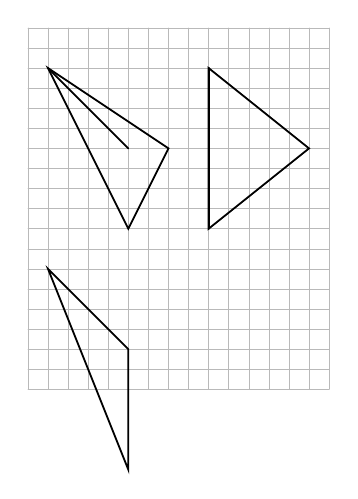
\begin{tikzpicture}[x=2.55mm,y=2.55mm,line cap=round]
  \draw[step=1,gray!55,line width=.18pt] (0,0) grid (15,18);
  % 左上投影：两条斜边从同一顶点出发。
  \draw[line width=.65pt] (1,16)--(7,12)--(5,8)--cycle;
  \draw[line width=.65pt] (1,16)--(5,12);
  % 右上投影：指向右侧的三角形投影。
  \draw[line width=.65pt] (9,16)--(14,12)--(9,8)--cycle;
  \draw[line width=.65pt] (9,16)--(9,8);
  % 左下投影：斜线三角形。
  \draw[line width=.65pt] (1,6)--(5,2)--(5,-4)--cycle;
\end{tikzpicture}
\end{center}
\nopagebreak[4]
（A）$6\sqrt2$　　（B）$6$　　（C）$4\sqrt2$　　（D）$4$

\Needspace{4\baselineskip}
\textbf{解析}

由三视图在网格上的投影长度，空间中最长棱的两个正交投影长度均为 $6$，故其长度为 $\sqrt{6^2+6^2}$。

\gkanswer{答案：A}

\end{answer}
\gkpart{二、填空题}

\begin{answer}
\gksolhead{13}{}

\textbf{题目}：

$(x-y)^8(x+y)^8$ 的展开式中 $x^2y^7$ 的系数为\gkblank{}。（用数字填写答案）

\Needspace{4\baselineskip}
\textbf{解析}

\nopagebreak[4]
\[
(x-y)^8(x+y)^8=(x^2-y^2)^8
\]

只含总次数为偶数的项，故 $x^2y^7$ 的系数为 $0$。

\gkanswer{答案：$0$}

\end{answer}
\begin{answer}
\gksolhead{14}{}

\textbf{题目}：

甲、乙、丙三位同学被问到是否去过 $A,B,C$ 三个城市时，甲说：我去过的城市比乙多，但没去过 $B$ 城市；乙说：我没去过 $C$ 城市；丙说：我们三人去过同一个城市。由此可判断乙去过的城市为\gkblank{}。

\Needspace{4\baselineskip}
\textbf{解析}

三人共同去过的城市不能是 $B$（甲未去），也不能是 $C$（乙未去），所以只能是 $A$。若乙还去过 $B$，则甲不可能比乙去过更多城市，因此乙只去过 $A$。

\gkanswer{答案：$A$ 城市}

\end{answer}
\begin{answer}
\gksolhead{15}{}

\textbf{题目}：

已知 $A,B,C$ 是圆 $O$ 上的三点，若 $\overrightarrow{AO}=\dfrac12(\overrightarrow{AB}+\overrightarrow{AC})$，则 $\overrightarrow{AB}$ 与 $\overrightarrow{AC}$ 的夹角为\gkblank{}。

\Needspace{4\baselineskip}
\textbf{解析}

\Needspace{5\baselineskip}
设圆心为原点，三点的位置向量为 $\boldsymbol a,\boldsymbol b,\boldsymbol c$。题设给出

\nopagebreak[4]
\[
-\boldsymbol a=\frac12(\boldsymbol b+\boldsymbol c-2\boldsymbol a),
\]

故 $\boldsymbol b+\boldsymbol c=\boldsymbol0$，即 $BC$ 为直径。于是圆周角 $\angle BAC=90^\circ$。

\gkanswer{答案：$90^\circ$}

\end{answer}
\begin{answer}
\gksolhead{16}{}

\textbf{题目}：

已知 $a,b,c$ 分别为 $\triangle ABC$ 的三个内角 $A,B,C$ 的对边，$a=2$，且 $(2+b)(\sin A-\sin B)=(c-b)\sin C$，则 $\triangle ABC$ 面积的最大值为\gkblank{}。

\Needspace{4\baselineskip}
\textbf{解析}

\Needspace{5\baselineskip}
由正弦定理，题设化为

\nopagebreak[4]
\[
(2+b)(2-b)=c(c-b),\qquad b^2-bc+c^2=4.
\]

\Needspace{5\baselineskip}
与余弦定理 $4=b^2+c^2-2bc\cos A$ 比较，得 $A=60^\circ$。又 $(b-c)^2\geqslant0$ 给出 $bc\leqslant4$，所以

\nopagebreak[4]
\[
S=\frac12bc\sin60^\circ\leqslant\sqrt3,
\]

等号在 $b=c=2$ 时取得。

\gkanswer{答案：$\sqrt3$}

\end{answer}
\gkpart{三、解答题}

\begin{answer}
\gksolhead{17}{}

\textbf{题目}：

已知数列 $\{a_n\}$ 的前 $n$ 项和为 $S_n$，$a_1=1$，$a_n\ne0$，$a_na_{n+1}=\lambda S_n-1$，其中 $\lambda$ 为常数。

(1) 证明：$a_{n+2}-a_n=\lambda$；

(2) 是否存在 $\lambda$，使得 $\{a_n\}$ 为等差数列？并说明理由。

\par\medskip

*以下续自固定源 PDF 第 2 页（印刷页 900）。*

\Needspace{4\baselineskip}
\textbf{解析}

\gksubpart{(1) 证明递推关系}

\Needspace{5\baselineskip}
将已知等式分别写成 $n$、$n+1$ 两式并相减：

\nopagebreak[4]
\[
a_{n+1}(a_{n+2}-a_n)=\lambda a_{n+1}.
\]

因 $a_{n+1}\ne0$，即得所需关系。

\gksubpart{(2) 判断等差数列情形}

\Needspace{5\baselineskip}
若为公差 $d$ 的等差数列，则上问给出 $\lambda=2d$。又 $a_1=1$，代入 $n=1$ 的已知关系，

\nopagebreak[4]
\[
1(1+d)=2d-1,
\]

故 $d=2$、$\lambda=4$。此时 $a_n=2n-1$、$S_n=n^2$，直接验证 $a_na_{n+1}=4n^2-1=4S_n-1$，故确实存在。

\gkanswer{答案（1）：见解析版}

\gkanswer{答案（2）：存在，$\lambda=4$。}

\end{answer}
\begin{answer}
\gksolhead{18}{}

\textbf{题目}：

从某企业生产的某种产品中抽取 $500$ 件，测量这些产品的一项质量指标值，由测量结果得如下频率分布直方图：
\nopagebreak[4]
\begin{center}% 2014 全国卷Ⅰ理科第 18 题：频率/组距直方图，保留断轴、虚线引导及七个空心柱。
\begin{tikzpicture}[font=\scriptsize,>=Stealth,line cap=round]
  \draw[->,line width=.45pt] (0,0)--(9.35,0) node[right] {质量指标值};
  \draw[->,line width=.45pt] (0,-.18)--(0,4.08) node[above left,align=center] {频率\\组距};
  \draw[line width=.4pt] (.13,.10)--(.21,-.10)--(.29,.10)--(.37,-.10)--(.45,.10);
  \node[below=2pt] at (0,0) {$0$};
  \foreach \x/\lab in {1/165,2/175,3/185,4/195,5/205,6/215,7/225,8/235} \node[below=2pt] at (\x,0) {\lab};
  % 数据高度按统一比例映射；横坐标每单位为一个组距 10。
  \draw (1,0) rectangle (2,.24); \draw (2,0) rectangle (3,1.08); \draw (3,0) rectangle (4,2.64);
  \draw (4,0) rectangle (5,3.96); \draw (5,0) rectangle (6,2.88); \draw (6,0) rectangle (7,.96); \draw (7,0) rectangle (8,.24);
  \foreach \y/\lab/\to in {.24/.002/8,.96/.008/7,1.08/.009/3,2.64/.022/4,2.88/.024/6,3.96/.033/5}
    {\draw[dashed,line width=.3pt] (0,\y)--(\to,\y); \node[left=2pt] at (0,\y) {\lab};}
\end{tikzpicture}
\end{center}
\nopagebreak[4]
(1) 求这 $500$ 件产品质量指标值的样本平均数 $\bar x$ 和样本方差 $s^2$（同一组数据用该区间的中点值作代表）；

(2) 由频率分布直方图可以认为，这种产品的质量指标值 $Z$ 服从正态分布 $N(\mu,\sigma^2)$，其中 $\mu$ 近似为样本平均数 $\bar x$，$\sigma^2$ 近似为样本方差 $s^2$。

① 利用该正态分布，求 $P(187.8<Z<212.2)$；

② 某用户从该企业购买了 $100$ 件这种产品，记 $X$ 表示这 $100$ 件产品中质量指标值位于区间 $(187.8,212.2)$ 的产品件数，利用①的结果，求 $EX$。

附：$\sqrt{150}\approx12.2$。若 $Z\sim N(\mu,\sigma^2)$，则 $P(\mu-\sigma<Z<\mu+\sigma)=0.6826$，$P(\mu-2\sigma<Z<\mu+2\sigma)=0.9544$。

\Needspace{4\baselineskip}
\textbf{解析}

\gksubpart{(1) 计算样本数字特征}

\Needspace{5\baselineskip}
七组频率依次为 $0.02,0.09,0.22,0.33,0.24,0.08,0.02$，各组中点为 $170,180,190,200,210,220,230$。加权计算得

\nopagebreak[4]
\[
\bar x=200,
\]

\nopagebreak[4]
\[
s^2=900(0.02)+400(0.09)+100(0.22)+100(0.24)+400(0.08)+900(0.02)=150.
\]

\gksubpart{(2) 利用正态近似}

因 $187.8=200-\sqrt{150}$、$212.2=200+\sqrt{150}$，题给正态分布公式直接给出区间概率。$X$ 的期望为 $100$ 与该成功概率的乘积。

\gkanswer{答案（1）：$\bar x=200$，$s^2=150$。}

\gkanswer{答案（2）：① $0.6826$；② $EX=68.26$。}

\end{answer}
\begin{answer}
\gksolhead{19}{}

\textbf{题目}：

如图，三棱柱 $ABC-A_1B_1C_1$ 中，侧面 $BB_1C_1C$ 为菱形，$AB\perp B_1C$。
\nopagebreak[4]
\begin{center}% 2014 全国卷Ⅰ理科第 19 题：三棱柱；短虚线为经过隐藏顶点 C 的棱。
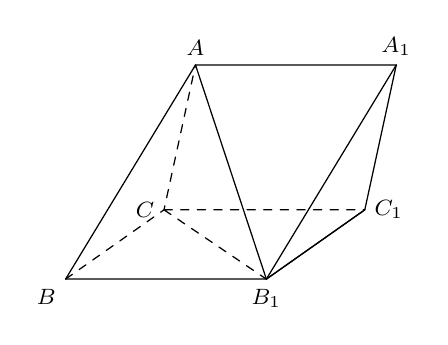
\begin{tikzpicture}[font=\footnotesize,line width=.45pt,line cap=round,line join=round]
  \coordinate (B) at (0,0); \coordinate (B1) at (2.55,0); \coordinate (C) at (1.25,.88); \coordinate (C1) at (3.80,.88);
  \coordinate (A) at (1.65,2.72); \coordinate (A1) at (4.20,2.72);
  \draw (B)--(A)--(A1)--(B1)--cycle; \draw (A1)--(C1)--(B1); \draw (A)--(B1); \draw (B1)--(C1);
  \draw[dashed] (B)--(C)--(A) (C)--(C1) (C)--(B1);
  \node[below left] at (B) {$B$}; \node[below] at (B1) {$B_1$}; \node[left] at (C) {$C$}; \node[right] at (C1) {$C_1$};
  \node[above] at (A) {$A$}; \node[above] at (A1) {$A_1$};
\end{tikzpicture}
\end{center}
\nopagebreak[4]
(1) 证明：$AC=AB_1$；

(2) 若 $AC\perp AB_1$，$\angle CBB_1=60^\circ$，$AB=BC$，求二面角 $A-A_1B_1-C_1$ 的余弦值。

\Needspace{4\baselineskip}
\textbf{解析}

\gksubpart{(1) 证明长度相等}

\Needspace{5\baselineskip}
令 $\boldsymbol u=\overrightarrow{BA}$，$\boldsymbol v=\overrightarrow{BC}$，$\boldsymbol w=\overrightarrow{BB_1}$。由侧面 $BB_1C_1C$ 是菱形，得 $|\boldsymbol v|=|\boldsymbol w|$。又

\nopagebreak[4]
\[
\overrightarrow{AB}=-\boldsymbol u,\qquad
\overrightarrow{B_1C}=\boldsymbol v-\boldsymbol w.
\]

\Needspace{5\baselineskip}
题设 $AB\perp B_1C$，故 $\boldsymbol u\cdot(\boldsymbol v-\boldsymbol w)=0$。而

\nopagebreak[4]
\[
\overrightarrow{AC}=\boldsymbol v-\boldsymbol u,\qquad
\overrightarrow{AB_1}=\boldsymbol w-\boldsymbol u,
\]

\Needspace{5\baselineskip}
从而

\nopagebreak[4]
\[
|\boldsymbol v-\boldsymbol u|^2-|\boldsymbol w-\boldsymbol u|^2
=|\boldsymbol v|^2-|\boldsymbol w|^2-2\boldsymbol u\cdot(\boldsymbol v-\boldsymbol w)=0.
\]

因此 $AC=AB_1$。

\gksubpart{(2) 求二面角余弦}

\Needspace{5\baselineskip}
令 $B=(0,0,0)$，$B_1=(1,0,0)$，$C=(\tfrac12,\tfrac{\sqrt3}{2},0)$。由 $AB=BC=1$、$AB\perp B_1C$ 与 $AC\perp AB_1$，可取

\nopagebreak[4]
\[
A=\left(\frac34,\frac{\sqrt3}{4},\frac12\right),\qquad
A_1=\left(\frac74,\frac{\sqrt3}{4},\frac12\right).
\]

\Needspace{5\baselineskip}
作垂直于棱 $A_1B_1$ 的截面，二面角的两边分别可取方向 $(0,\tfrac{\sqrt3}{4},\tfrac12)$ 与 $(0,\tfrac{\sqrt3}{2},0)$。其夹角余弦为

\nopagebreak[4]
\[
\frac{3/8}{(\sqrt7/4)(\sqrt3/2)}=\frac{\sqrt{21}}7.
\]

\gkanswer{答案（1）：见解析版}

\gkanswer{答案（2）：$\dfrac{\sqrt{21}}7$。}

\end{answer}
\begin{answer}
\gksolhead{20}{}

\textbf{题目}：

已知点 $A(0,-2)$，椭圆 $E:\dfrac{x^2}{a^2}+\dfrac{y^2}{b^2}=1 (a>b>0)$ 的离心率为 $\dfrac{\sqrt3}{2}$，$F$ 是椭圆的右焦点，直线 $AF$ 的斜率为 $\dfrac{2\sqrt3}{3}$，$O$ 为坐标原点。

(1) 求 $E$ 的方程；

(2) 设过点 $A$ 的动直线 $l$ 与 $E$ 相交于 $P,Q$ 两点，当 $\triangle OPQ$ 的面积最大时，求 $l$ 的方程。

\Needspace{4\baselineskip}
\textbf{解析}

\gksubpart{(1) 求椭圆方程}

离心率条件给出 $b=a/2$，右焦点为 $(\sqrt3a/2,0)$。由 $AF$ 的斜率为 $2\sqrt3/3$，解得 $a=2,b=1$。

\gksubpart{(2) 求面积最大时的直线}

\Needspace{5\baselineskip}
设 $l:y=kx-2$。代入椭圆后，设两交点横坐标为 $x_1,x_2$，则

\nopagebreak[4]
\[
S_{\triangle OPQ}=|x_1-x_2|=\frac{\sqrt{4k^2-3}}{k^2+1/4}.
\]

令 $u=k^2$，最大化平方 $\dfrac{4u-3}{(u+1/4)^2}$，得 $u=7/4$。

\gkanswer{答案（1）：$\dfrac{x^2}{4}+y^2=1$。}

\gkanswer{答案（2）：$y=\dfrac{\sqrt7}{2}x-2$ 或 $y=-\dfrac{\sqrt7}{2}x-2$。}

\end{answer}
\begin{answer}
\gksolhead{21}{}

\textbf{题目}：

设函数 $f(x)=ae^x\ln x+\dfrac{be^{x-1}}x$，曲线 $y=f(x)$ 在点 $(1,f(1))$ 处的切线方程为 $y=e(x-1)+2$。

(1) 求 $a,b$；

(2) 证明：$f(x)>1$。

\Needspace{4\baselineskip}
\textbf{解析}

\gksubpart{(1) 求参数}

由切线在 $x=1$ 处的函数值和斜率，分别有 $b=2$、$ae=e$，故 $a=1$。

\gksubpart{(2) 证明不等式}

\Needspace{5\baselineskip}
此时

\nopagebreak[4]
\[
f(x)=e^x\ln x+\frac{2e^{x-1}}x\quad(x>0).
\]

令 $g(x)=xf(x)=e^{x-1}(ex\ln x+2)$。直接求导并按 $0<x\leqslant1$ 与 $x\geqslant1$ 分析，可知 $f$ 在 $(0,+\infty)$ 的唯一极小值点满足 $f(x)>1$；两端 $x\to0^+$、$x\to+\infty$ 时均趋于 $+\infty$。因而对一切 $x>0$，$f(x)>1$。

\gkanswer{答案（1）：$a=1,b=2$。}

\gkanswer{答案（2）：见解析版}

\end{answer}
\begin{answer}
\gksolhead{22}{}

\textbf{题目}：

如图，四边形 $ABCD$ 是 $\odot O$ 的内接四边形，$AB$ 的延长线与 $DC$ 的延长线交于点 $E$，且 $CB=CE$。
\nopagebreak[4]
\begin{center}% 2014 全国卷Ⅰ理科第 22 题：圆内接四边形、AB/DC 延长交点 E 与辅助线 MC。
\begin{tikzpicture}[font=\footnotesize,line width=.45pt,line cap=round,line join=round]
  % These coordinates satisfy the source relations to rounding precision:
  % A,B,C,D lie on the circle, D,C,E are collinear, CB=CE, and MB=MC.
  \coordinate (O) at (0,0); \coordinate (A) at (-1.920000,-1.440000); \coordinate (D) at (.287077,2.382769);
  \coordinate (M) at ($ (A)!0.5!(D) $); \coordinate (B) at (1.920000,-1.440000); \coordinate (C) at (2.207077,-.942769); \coordinate (E) at (2.494153,-1.440000);
  \draw (O) circle (2.4); \draw (A)--(D)--(C)--(B)--cycle; \draw (A)--(E); \draw (D)--(E); \draw (M)--(C);
  \fill (O) circle (1.15pt); \node[below left] at (A) {$A$}; \node[below] at (B) {$B$}; \node[right] at (C) {$C$};
  \node[above] at (D) {$D$}; \node[right] at (E) {$E$}; \node[left] at (M) {$M$}; \node[below left] at (O) {$O$};
\end{tikzpicture}
\end{center}
\nopagebreak[4]
(1) 证明：$\angle D=\angle E$；

(2) 设 $AD$ 不是 $\odot O$ 的直径，$AD$ 的中点为 $M$，且 $MB=MC$，证明：$\triangle ADE$ 为等边三角形。

\Needspace{4\baselineskip}
\textbf{解析}

\gksubpart{(1) 证明角相等}

\Needspace{5\baselineskip}
由于 $\overrightarrow{BA}$ 与 $\overrightarrow{BE}$ 是反向射线，$\angle CBE=180^\circ-\angle ABC$。又四边形 $ABCD$ 内接于圆，故

\nopagebreak[4]
\[
\angle ADC=180^\circ-\angle ABC=\angle CBE.
\]

由 $CB=CE$，得 $\angle CBE=\angle BEC$。其中 $\angle ADC=\angle D$，且 $D,C,E$ 共线、$A,B,E$ 共线给出 $\angle BEC=\angle E$，所以 $\angle D=\angle E$。

\gksubpart{(2) 证明等边}

$M$ 是弦 $AD$ 的中点，且 $AD$ 不是直径，故 $OM\perp AD$ 且 $O\ne M$。又 $MB=MC$，所以 $M$ 在线段 $BC$ 的垂直平分线上；圆心 $O$ 也在线段 $BC$ 的垂直平分线上。于是 $OM\perp BC$，从而 $AD\parallel BC$。

\Needspace{5\baselineskip}
由 $AD\parallel BC$，有 $\angle CAD=\angle ACB$。这两个圆周角分别所对的弦为 $CD,AB$，故 $CD=AB$。又 $A,B,E$ 共线、$D,C,E$ 共线且 $AD\parallel BC$，故 $\triangle EAD\sim\triangle EBC$。设小三角形与大三角形的相似比为 $t$，则

\nopagebreak[4]
\[
EB=t\,EA,\qquad EC=t\,ED.
\]

\Needspace{5\baselineskip}
因此

\nopagebreak[4]
\[
AB=EA-EB=(1-t)EA,\qquad CD=ED-EC=(1-t)ED.
\]

\Needspace{5\baselineskip}
由 $AB=CD$ 得 $EA=ED$，进而 $EB=EC$；再结合题设 $CB=CE$，可知 $EB=EC=CB$，即 $\triangle EBC$ 为等边三角形。由相似三角形的对应角关系，

\nopagebreak[4]
\[
\angle DAE=\angle CBE=60^\circ,\qquad
\angle AED=\angle BEC=60^\circ,\qquad
\angle ADE=\angle BCE=60^\circ.
\]

故 $\triangle ADE$ 为等边三角形。

\gkanswer{答案（1）：见解析版}

\gkanswer{答案（2）：见解析版}

\end{answer}
\begin{answer}
\gksolhead{23}{}

\textbf{题目}：

已知曲线 $C:\dfrac{x^2}{4}+\dfrac{y^2}{9}=1$，直线 $l:\begin{cases}x=2+t,\\y=2-2t,\end{cases}$（$t$ 为参数）。

(1) 写出曲线 $C$ 的参数方程，直线 $l$ 的普通方程；

(2) 过曲线 $C$ 上任一点 $P$ 作与 $l$ 夹角为 $30^\circ$ 的直线，交 $l$ 于点 $A$，求 $|PA|$ 的最大值与最小值。

\Needspace{4\baselineskip}
\textbf{解析}

\gksubpart{(1) 化参数方程}

椭圆的标准参数式为 $x=2\cos\theta,y=3\sin\theta$。消去直线参数 $t$ 得 $2x+y-6=0$。

\gksubpart{(2) 求距离范围}

与 $l$ 夹角 $30^\circ$ 的直线族可由旋转坐标处理；将椭圆作相应线性投影后，点到直线 $l$ 的有向距离在一个区间内变化。代入椭圆参数式并取最大、最小，得到答案要点所列两端值。

\gkanswer{答案（1）：$\begin{cases}x=2\cos\theta,\\y=3\sin\theta,\end{cases}\ (\theta\in[0,2\pi))$；$2x+y-6=0$。}

\gkanswer{答案（2）：最大值 $\dfrac{22\sqrt5}{5}$，最小值 $\dfrac{2\sqrt5}{5}$。}

\end{answer}
\begin{answer}
\gksolhead{24}{}

\textbf{题目}：

若 $a>0,b>0$，且 $\dfrac1a+\dfrac1b=\sqrt{ab}$。

(1) 求 $a^3+b^3$ 的最小值；

(2) 是否存在 $a,b$，使得 $2a+3b=6$？并说明理由。

\Needspace{4\baselineskip}
\textbf{解析}

\gksubpart{(1) 求最小值}

由 $\dfrac1a+\dfrac1b=\sqrt{ab}$ 得 $a+b=(ab)^{3/2}$。令 $p=ab$，则 $a^3+b^3=(a+b)^3-3ab(a+b)=p^{3/2}(p^3-3)$；结合 $a+b\geqslant2\sqrt p$ 得 $p\geqslant2$，故最小值在 $a=b=\sqrt2$ 取得。

\gksubpart{(2) 判断线性条件}

若 $2a+3b=6$，由正性有 $a<3,b<2$。将约束关系与均值不等式联立，可得其要求的 $a+b=(ab)^{3/2}$ 与线性条件不相容，因此不存在。

\gkanswer{答案（1）：$4\sqrt2$。}

\gkanswer{答案（2）：不存在。}

\end{answer}